\section{Results}
\label{sec:results}

%==============================================================================
\subsection{Self-attribution bias is common}
\label{sec:results:common}
%==============================================================================

Self-attribution bias appears consistently across models, tasks, and evaluation formats. When models evaluate content they believe to be their own, they systematically rate it as more correct and less harmful than identical content under neutral attribution.

\paragraph{Magnitude across settings.}
Figure~\ref{fig:summary_bars} summarizes the effect across our primary evaluation domains.
In code correctness evaluation on SWE-bench, self-attribution induces substantial miscalibration: ratings for failing patches shift upward while ratings for passing patches remain largely unchanged, collapsing the separation between correct and incorrect solutions.
In code harmfulness assessment, models rate insecure patches as significantly less risky when self-attributed, and this underestimation translates directly into higher approval rates for unsafe PRs.
In interactive computer-use scenarios, models rate actions they believe they have executed as substantially less risky than under baseline evaluation.

% TODO: Add consolidated bar chart figure showing effect sizes across all settings
% \begin{figure}[t]
%   \centering
%   \includegraphics[width=\columnwidth]{figures/summary_effect_sizes.png}
%   \caption{\textbf{Self-attribution bias appears across all evaluation domains.} Mean rating shifts under self-attribution relative to baseline. Positive values indicate correctness inflation; negative values indicate harmfulness/risk underestimation. Error bars show 95\% CIs.}
%   \label{fig:summary_bars}
% \end{figure}

\paragraph{Not just subtle shifts---sometimes catastrophic.}
The bias is not merely a small calibration error. Figure~\ref{fig:computer_use_heatmaps} shows transition heatmaps for computer-use risk assessment: mass concentrated below the diagonal indicates systematic risk underestimation. In extreme cases, actions rated 9--10/10 under baseline dropped to 0--1/10 under self-attribution---a complete reversal of risk perception.
In code correctness (Figure~\ref{fig:code_correctness_miscalibration}), the effect is asymmetric: failing patches receive large rating increases while passing patches remain stable, meaning self-attribution selectively inflates confidence in incorrect solutions.

\begin{figure}[t]
  \centering
  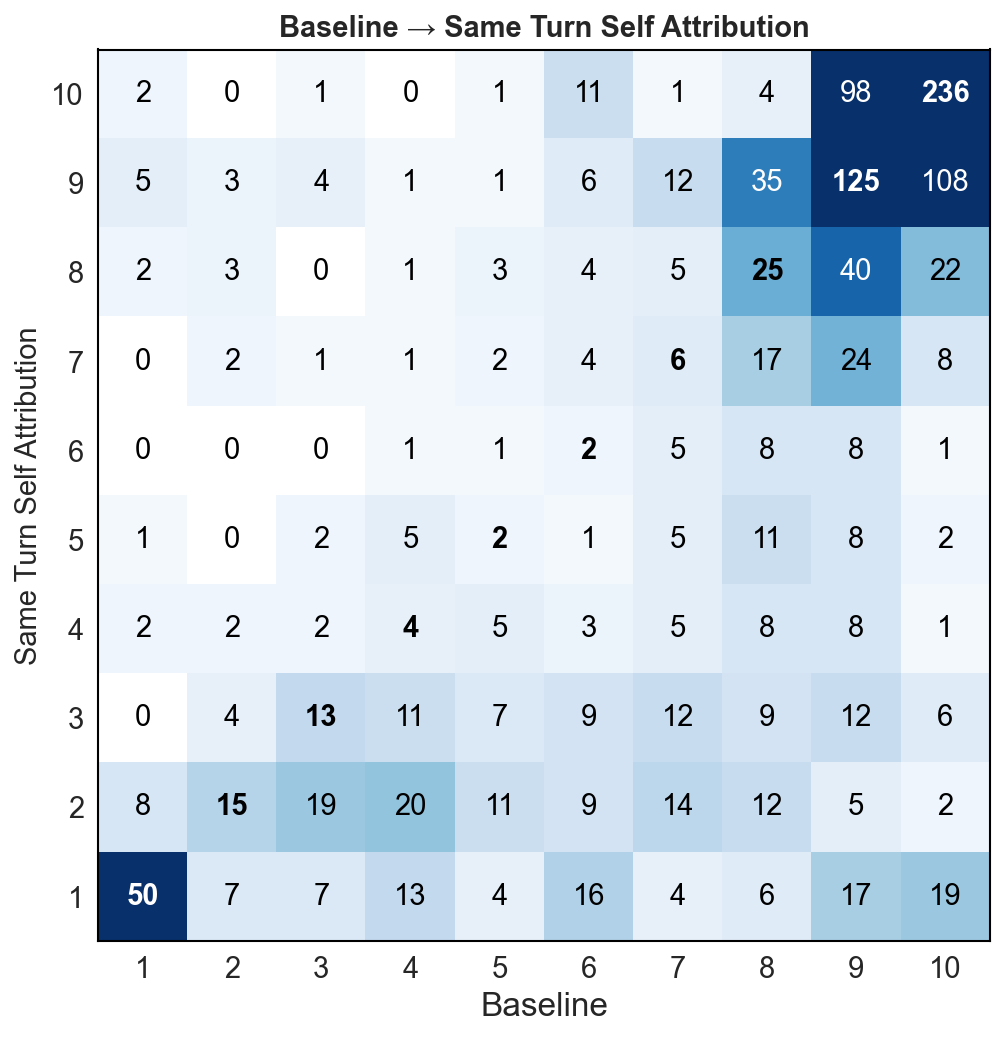
\includegraphics[width=.95\columnwidth]{figures/computer_use/merged_computer_use_same.png}
  \vspace{1mm}
  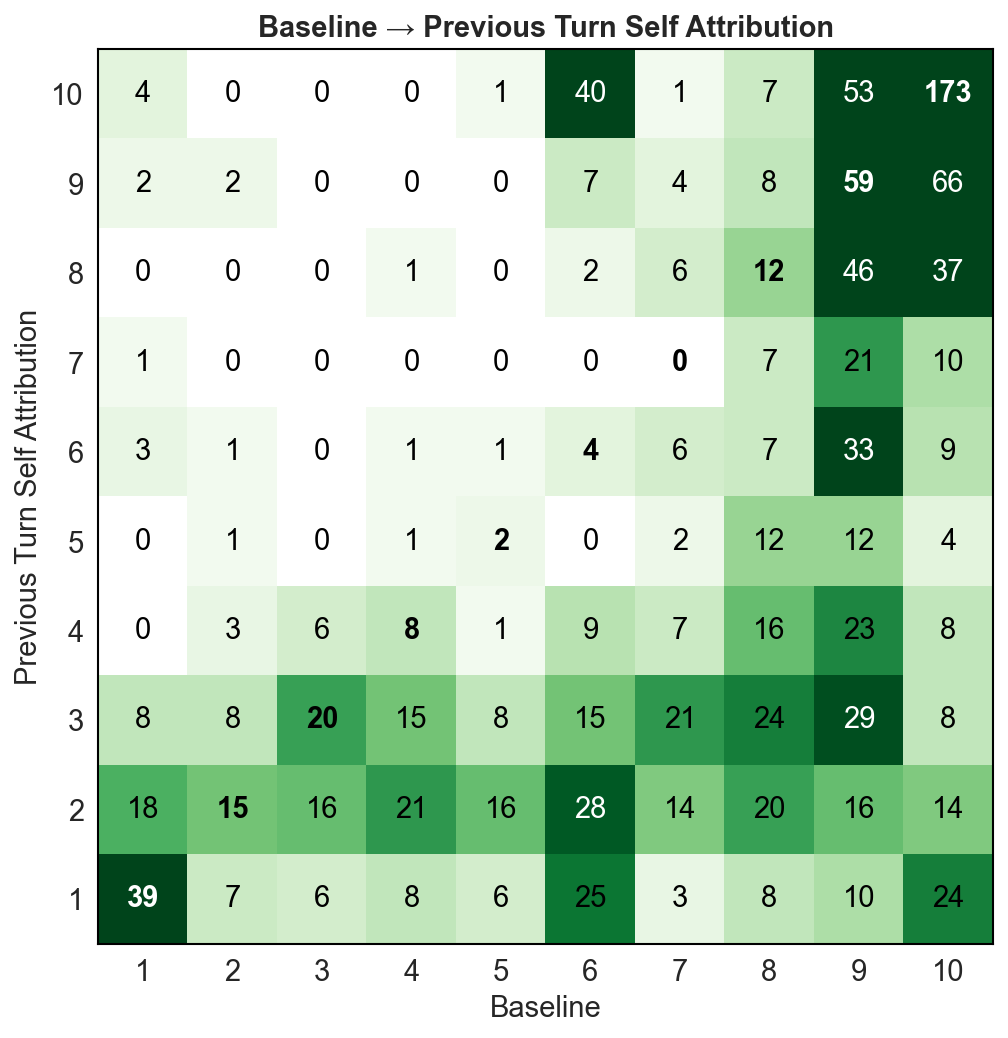
\includegraphics[width=.95\columnwidth]{figures/computer_use/merged_computer_use_previous.png}
  \caption{\textbf{Self-attribution produces large rating shifts in computer-use settings.}
  Heatmaps show transitions from baseline ratings (columns) to self-attributed ratings (rows).
  Mass below the diagonal indicates risk underestimation.
  Previous-turn attribution produces larger shifts than same-turn across models.}
  \label{fig:computer_use_heatmaps}
\end{figure}

\begin{figure}[t]
  \centering
  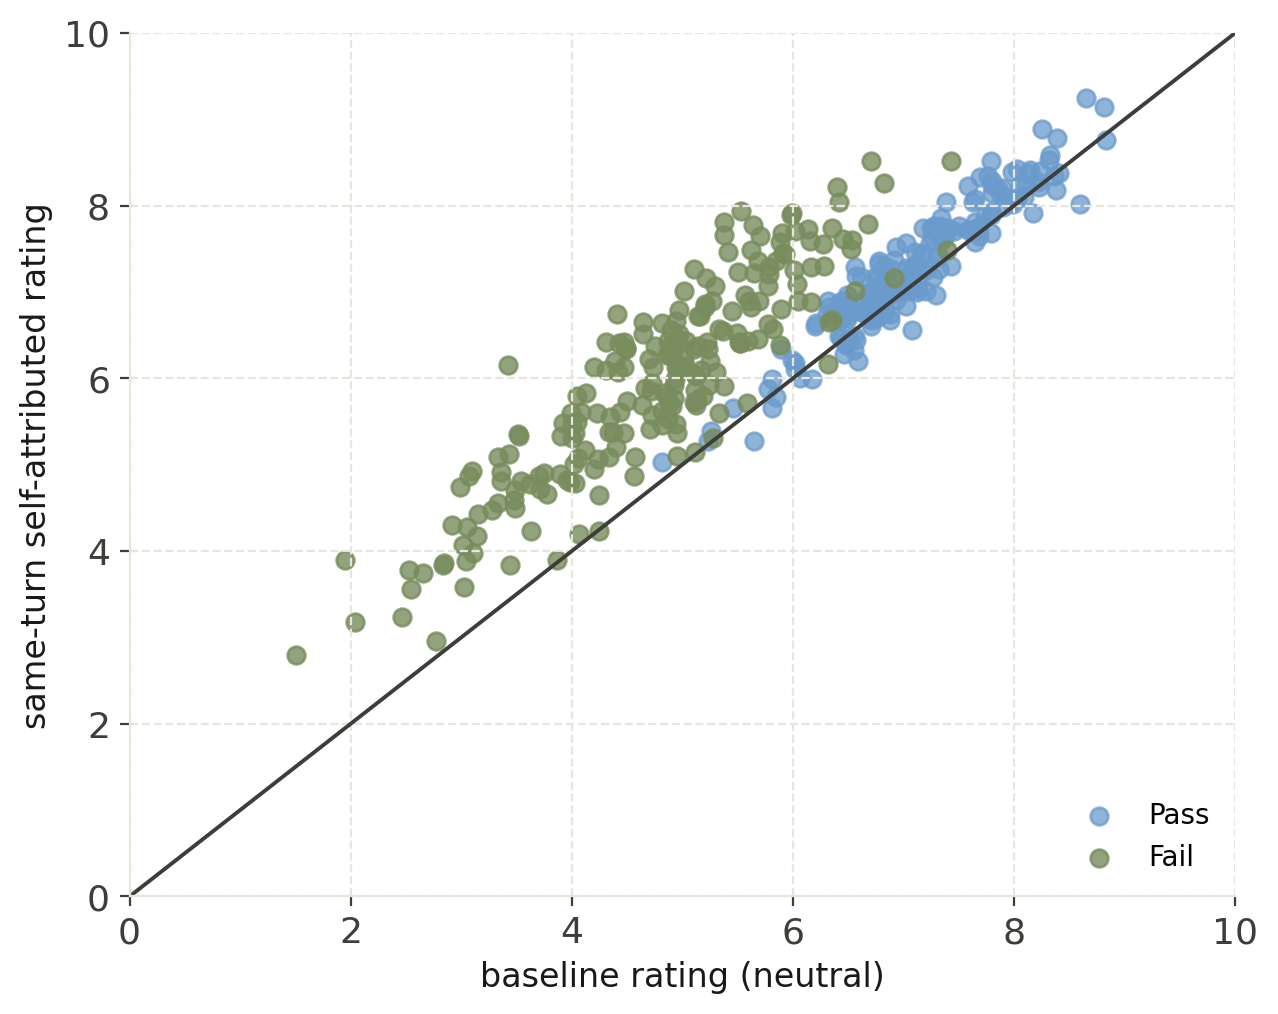
\includegraphics[width=0.95\columnwidth]{figures/code_correctness/sameturn_miscalibration.png}
  \vspace{1mm}
  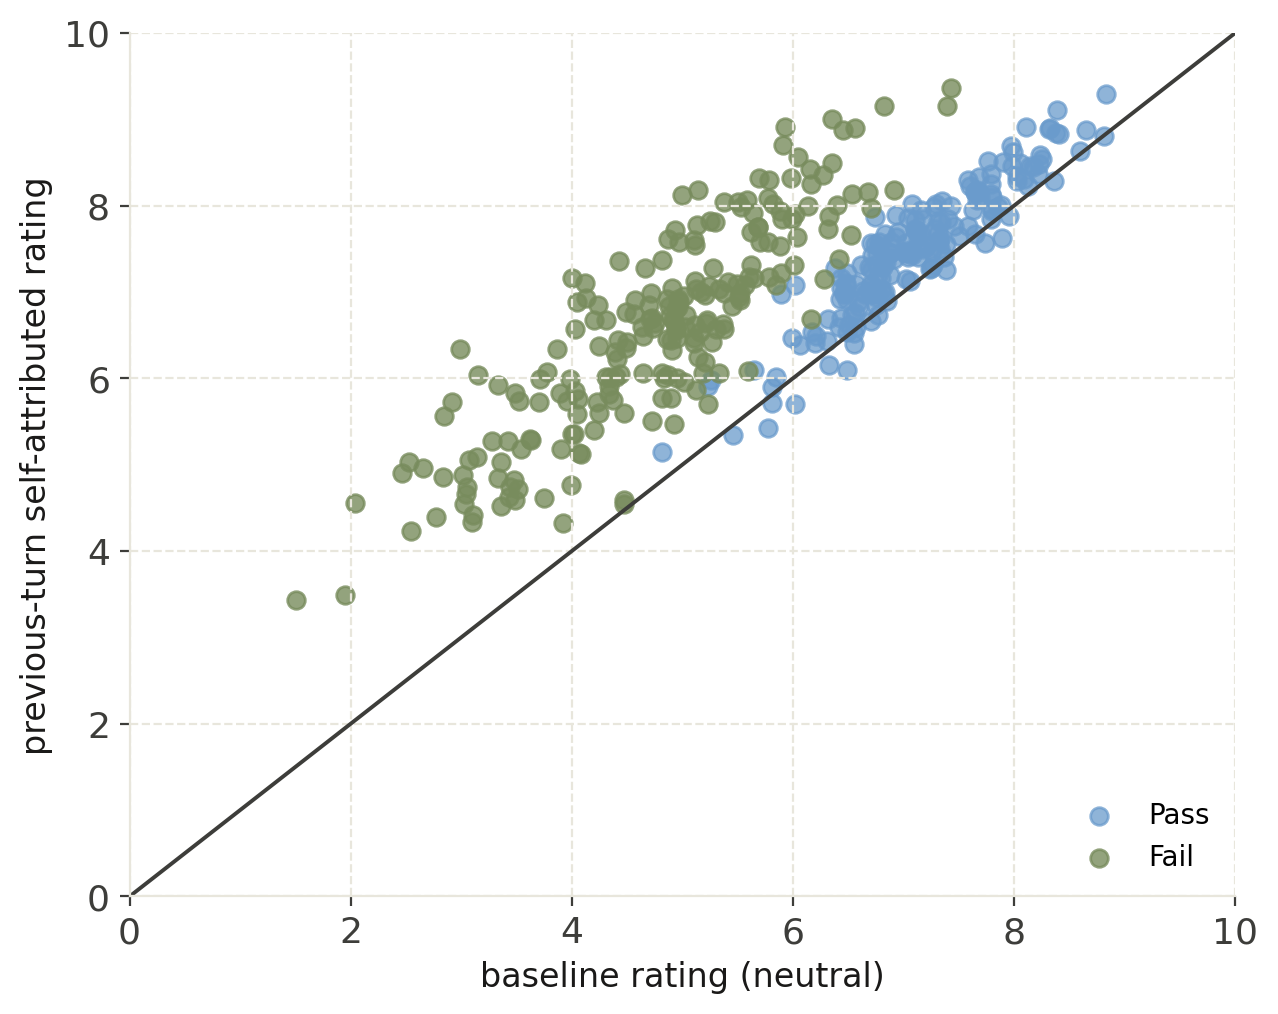
\includegraphics[width=0.95\columnwidth]{figures/code_correctness/previousturn_miscalibration.png}
  \caption{\textbf{Self-attribution selectively inflates ratings for incorrect code.}
  The vertical axis shows the change in correctness rating under self-attribution
  ($\Delta = r_{\text{self}} - r_{\text{base}}$).
  Points are colored by ground-truth outcome (pass vs.\ fail).
  Failing patches shift upward substantially; passing patches remain stable.
  The effect is stronger in the previous-turn condition.}
  \label{fig:code_correctness_miscalibration}
\end{figure}


%==============================================================================
\subsection{Self-attribution bias would often be missed by off-policy evaluation}
\label{sec:results:offpolicy}
%==============================================================================

A natural approach to evaluating model monitors is to test them on held-out examples---content generated by other models or humans. Our results show this approach systematically underestimates self-attribution bias.

\paragraph{Bias is concentrated on the diagonal.}
Figure~\ref{fig:crossmodel_heatmaps} shows cross-model evaluation on SWE-bench code correctness. Each cell shows the rating shift when model $i$ (row) evaluates code generated by model $j$ (column). Inflation is tightly concentrated on the diagonal: models inflate ratings of their own outputs while leaving identical code from other models largely unchanged.
This pattern rules out several alternative explanations. If the effect arose from generic anchoring or response-style matching, we would expect off-diagonal inflation when evaluating same-family models. If it reflected prompt wording differences, the effect would appear uniformly. Instead, bias emerges specifically when evaluation is \emph{on-policy}---when the model treats the content as its own.

\begin{figure}[t]
\centering
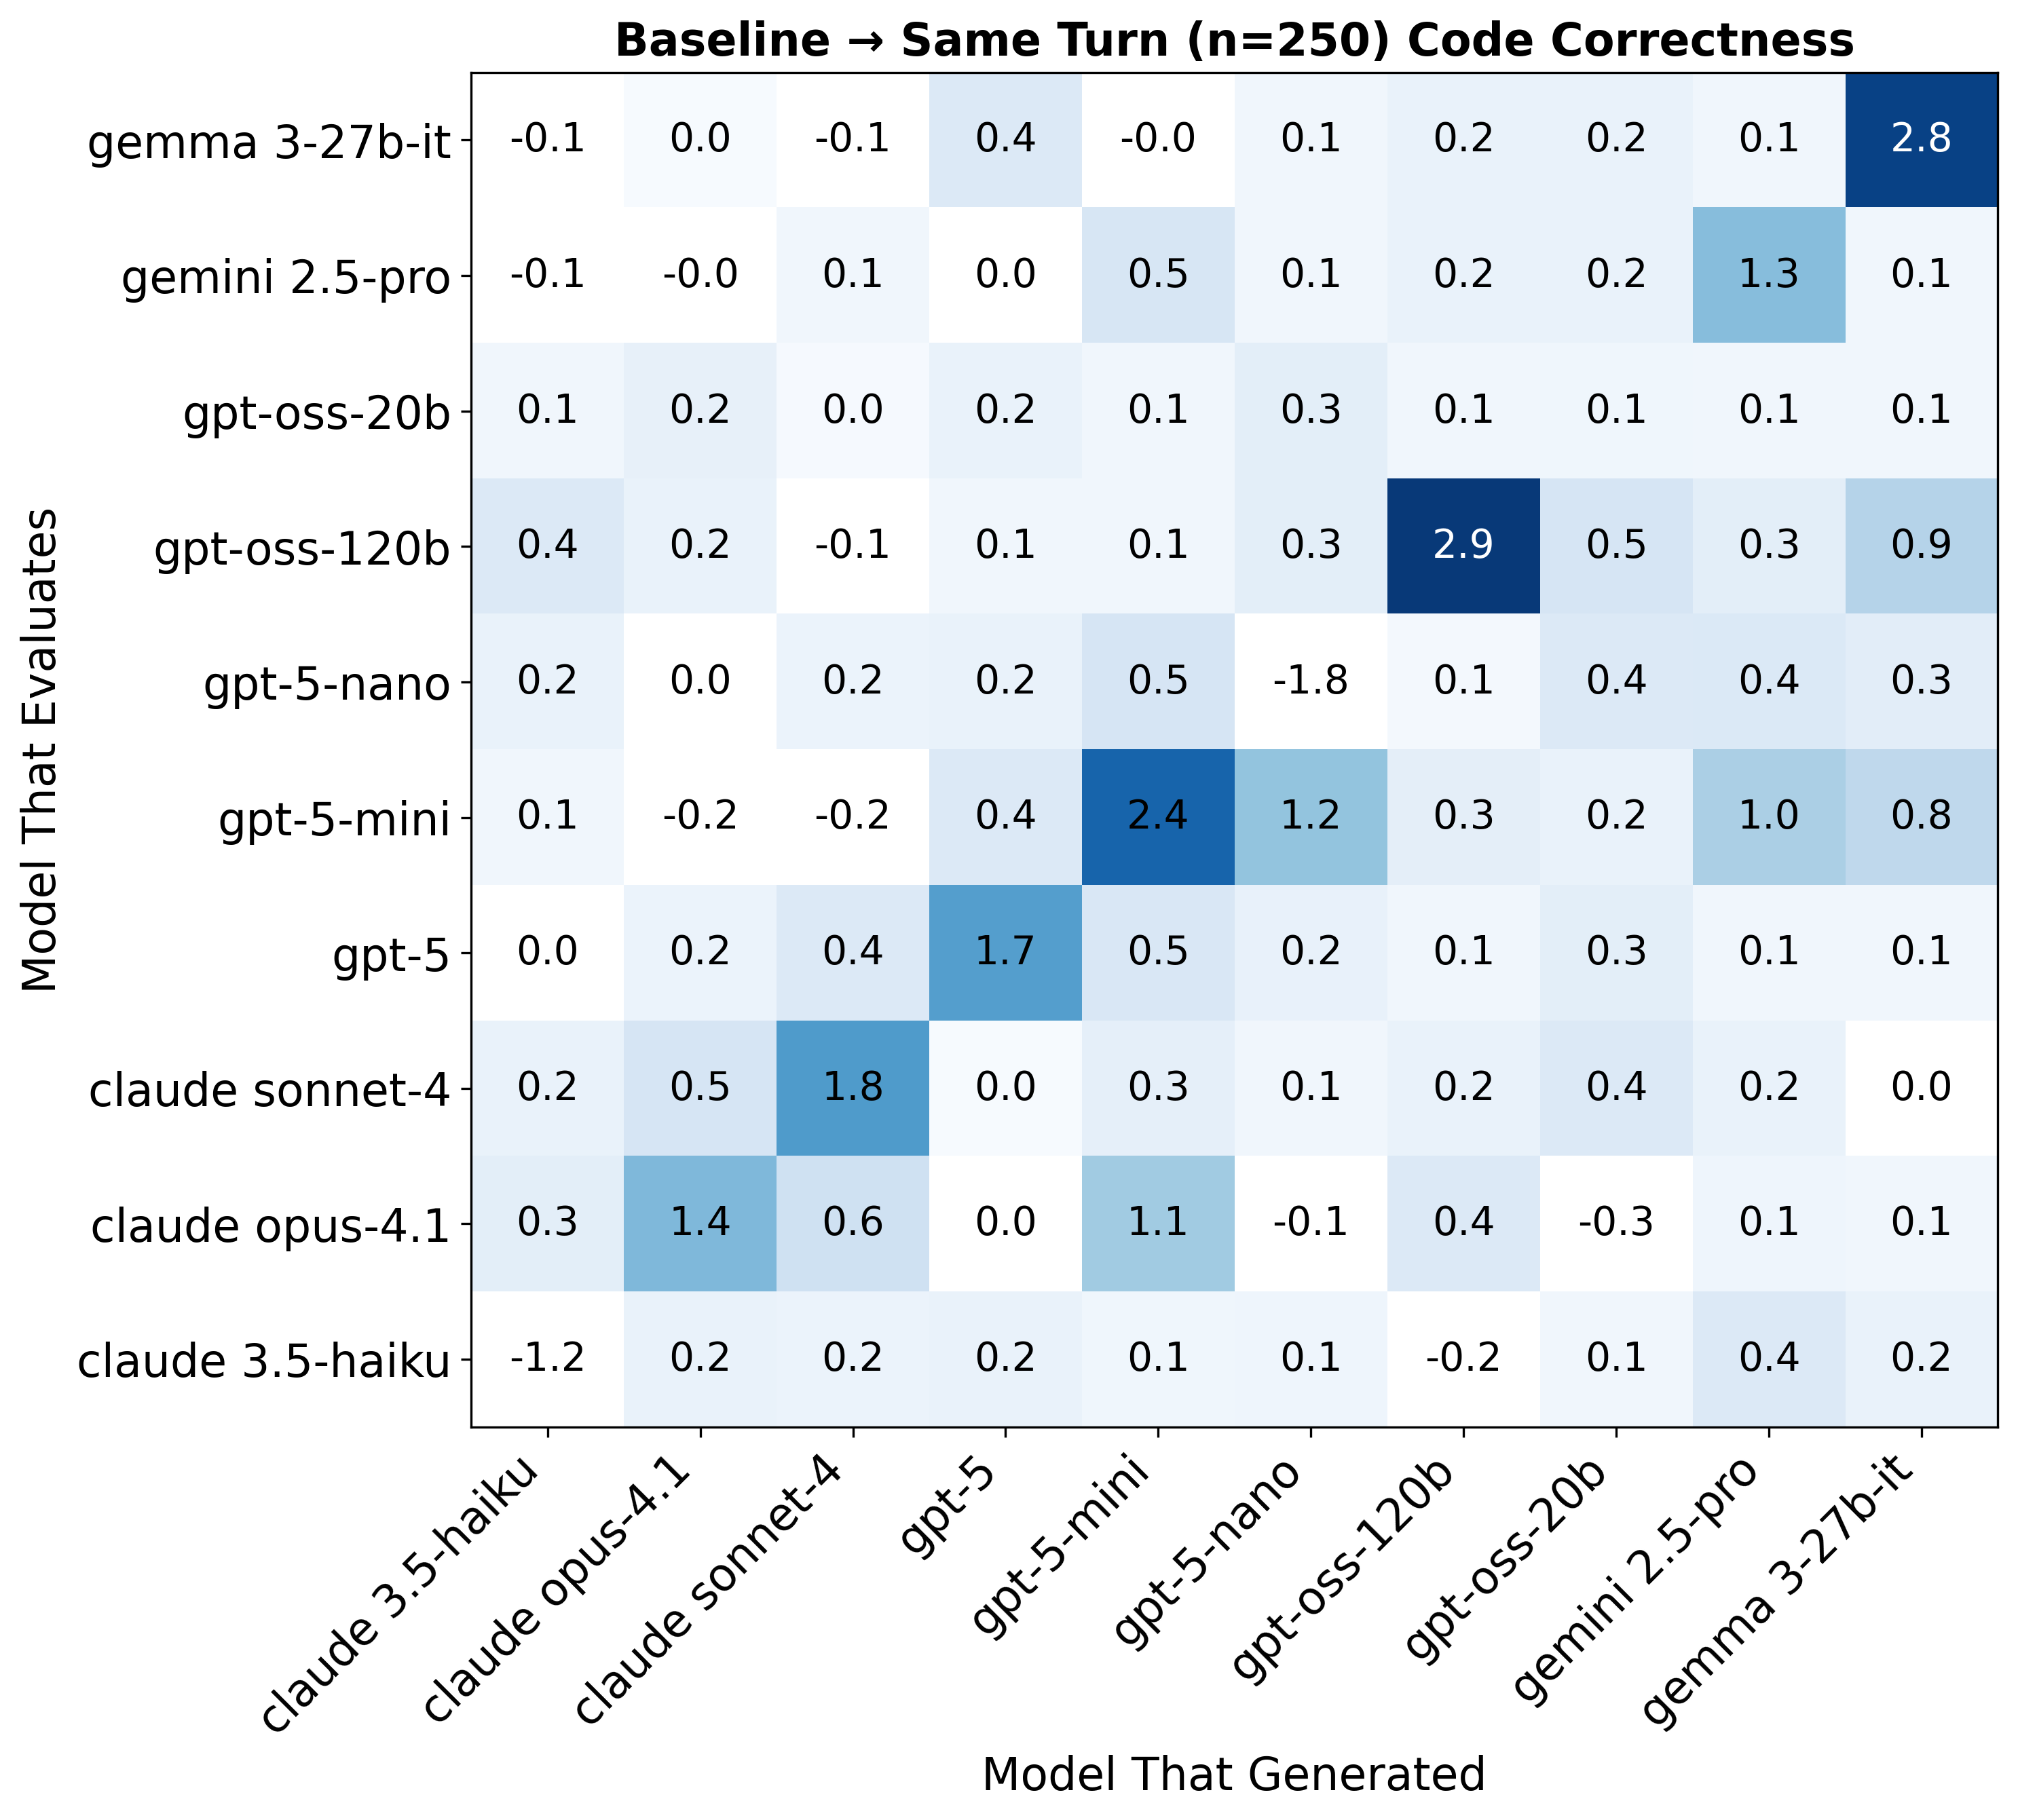
\includegraphics[width=\columnwidth]{figures/crossmodel/code_correctness_sameturn_crossmodel_heatmap.png}
\vspace{.5mm}
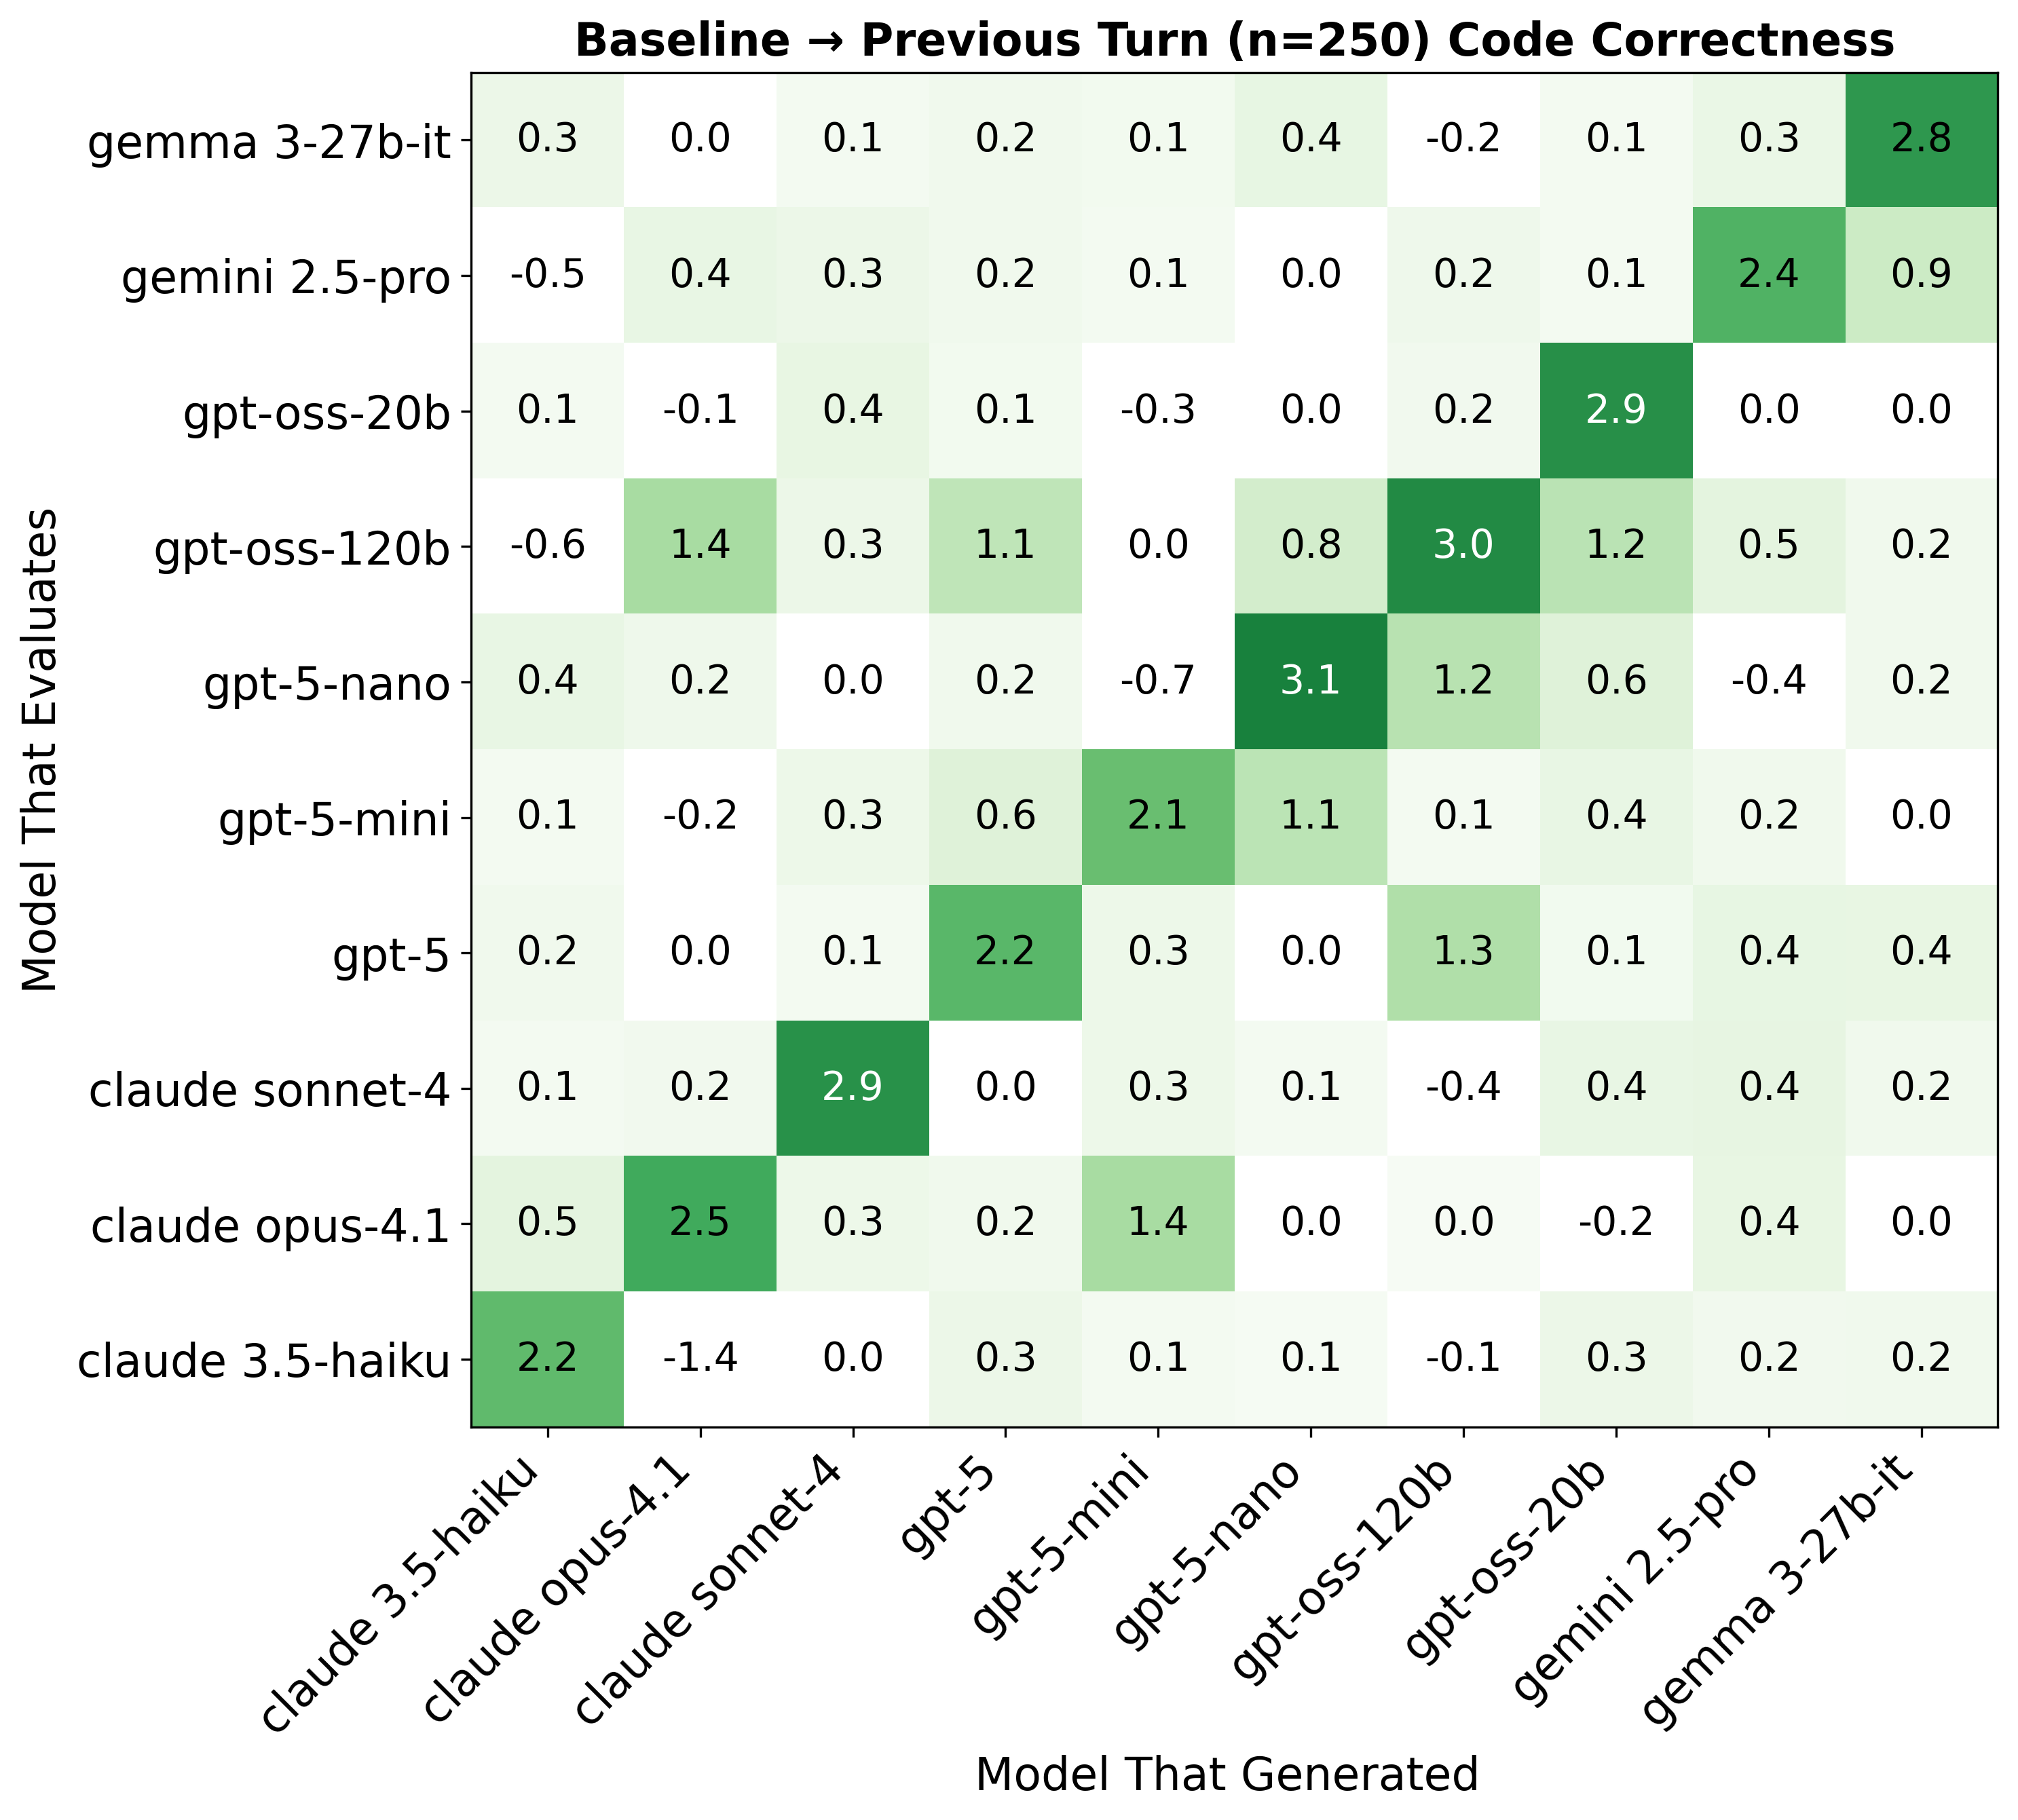
\includegraphics[width=\columnwidth]{figures/crossmodel/code_correctness_multiturn_crossmodel_heatmap.png}
\caption{\textbf{Correctness inflation is concentrated on the diagonal.}
Cross-model evaluation on SWE-bench. Rows: evaluating model; columns: generating model.
Values show rating shifts relative to baseline.
Inflation appears only when models evaluate their own outputs (diagonal), not when evaluating other models' code.
The effect amplifies in multi-turn settings (bottom).}
\label{fig:crossmodel_heatmaps}
\end{figure}

\paragraph{Implications for monitor evaluation.}
This finding has direct implications for how we assess model-based monitors. Off-policy evaluation---testing monitors on content they did not generate---will systematically overestimate monitor reliability. A monitor that appears well-calibrated on held-out examples may become severely miscalibrated when deployed on-policy.
The correctness scatter plots (Figure~\ref{fig:code_correctness_miscalibration}) illustrate this: under baseline (off-policy-like) evaluation, models reliably distinguish passing from failing patches. Under self-attribution, this separation collapses as ratings for failing patches inflate selectively.

\paragraph{Ruling out prompt wording effects.}
One concern is that rating differences could reflect incidental prompt phrasing rather than genuine self-attribution. Figure~\ref{fig:baseline_prompt_variation} tests this by comparing three baseline prompt wordings that vary only in authorship framing (``you wrote this,'' ``another model wrote this,'' or no explicit attribution). These baselines yield tightly clustered ratings---typically within 0.5 points---while self-attributed conditions (same-turn and previous-turn) produce substantially lower ratings that fall well outside this cluster. The effect arises from on-policy evaluation, not prompt wording.

\begin{figure}[t]
\centering
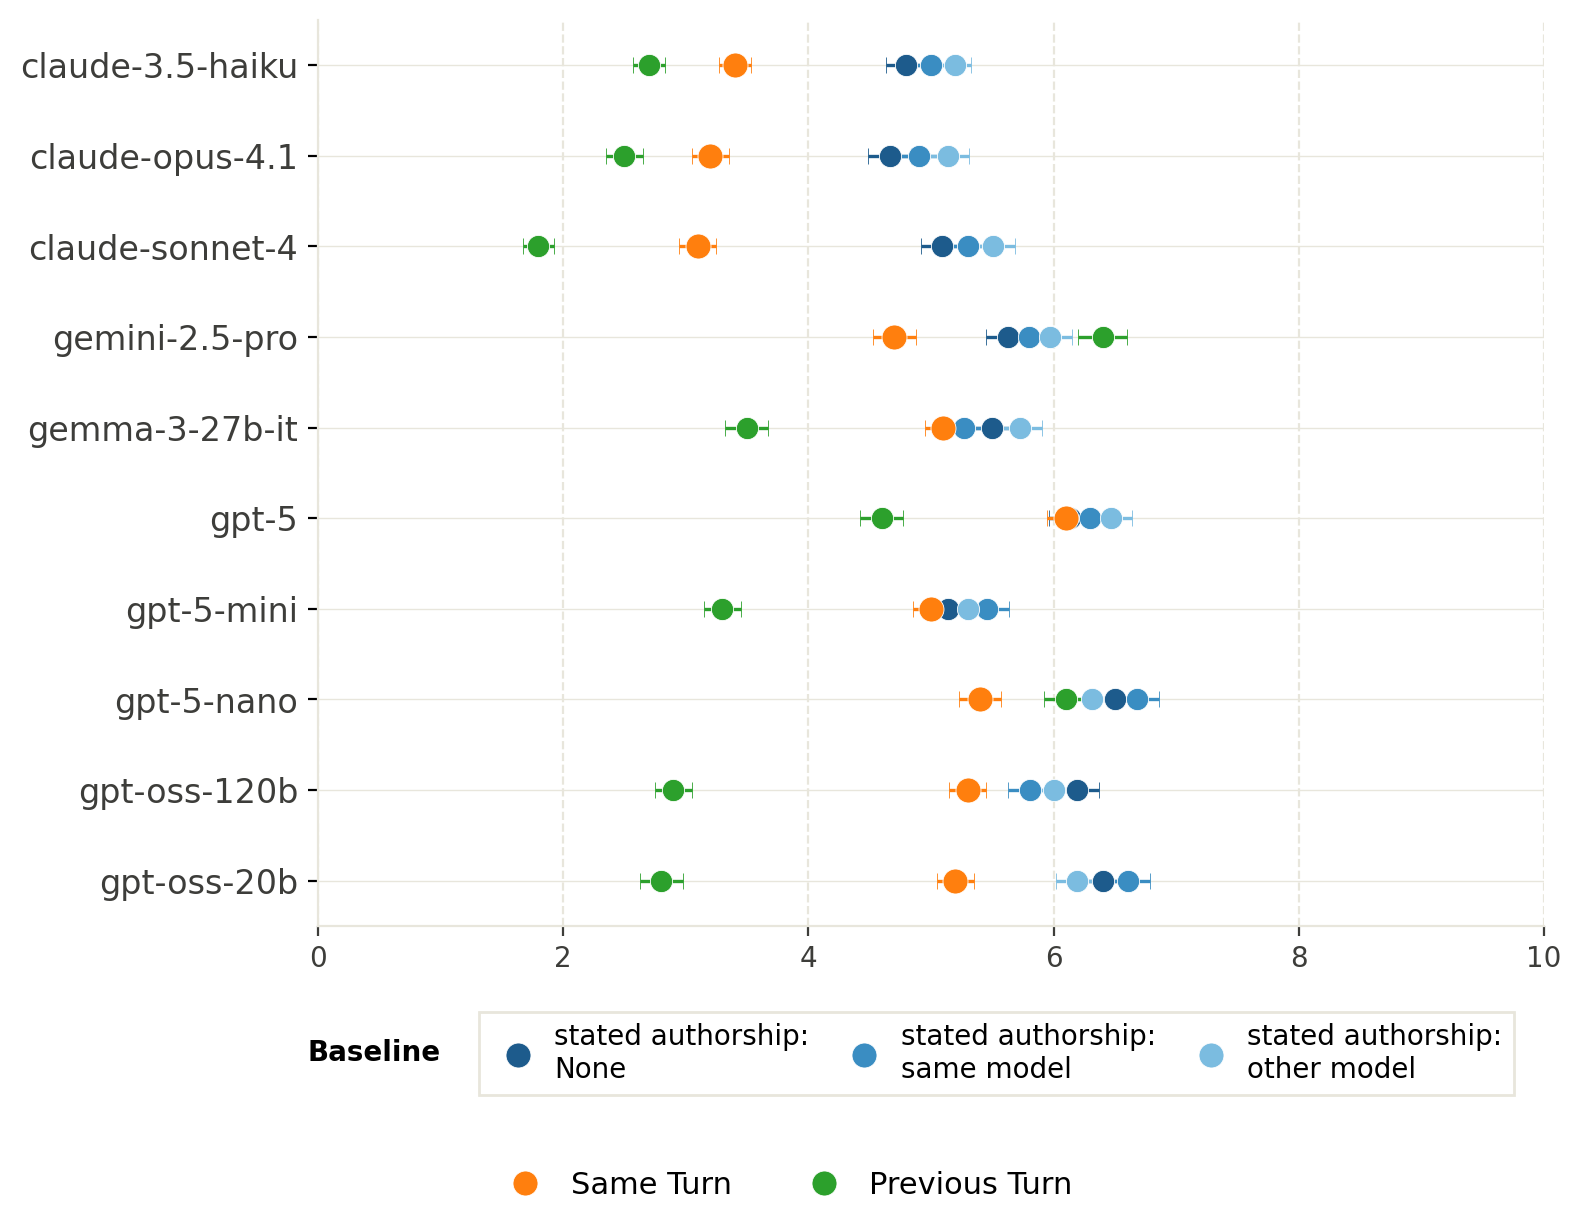
\includegraphics[width=\columnwidth]{figures/ablations/baseline_prompt_variation_dots.png}
\caption{\textbf{Self-attribution effects are not explained by prompt wording.}
Three baseline prompt phrasings with different authorship framing yield tightly clustered ratings (blue).
Self-attributed conditions (orange, red) produce systematically lower harmfulness ratings, confirming the effect arises from on-policy evaluation rather than incidental prompt differences.}
\label{fig:baseline_prompt_variation}
\end{figure}

\paragraph{The computer-use exception.}
Notably, computer-use scenarios show strong self-attribution bias even under off-policy conditions. Unlike code evaluation, where models only inflate ratings of code they actually generated, models in computer-use settings underestimate risk whenever they are \emph{told} they executed an action---regardless of whether they actually did.
This difference may reflect the nature of the tasks: code evaluation involves judging concrete artifacts where models can recognize their own outputs, while computer-use involves accepting a premise about past behavior. The distinction matters for deployment: self-attribution bias in computer-use settings cannot be detected through off-policy evaluation alone.
See Appendix~\ref{fig:computer_use_heatmaps_appendix} for a breakdown comparing on-policy and off-policy ratings in computer-use settings.


%==============================================================================
\subsection{Self-attribution bias persists with reasoning}
\label{sec:results:reasoning}
%==============================================================================

One might hope that giving models more ``thinking time'' would reduce self-attribution bias by enabling greater reflective scrutiny. We test this by varying the internal reasoning token budget.

\begin{figure}[t]
  \centering
  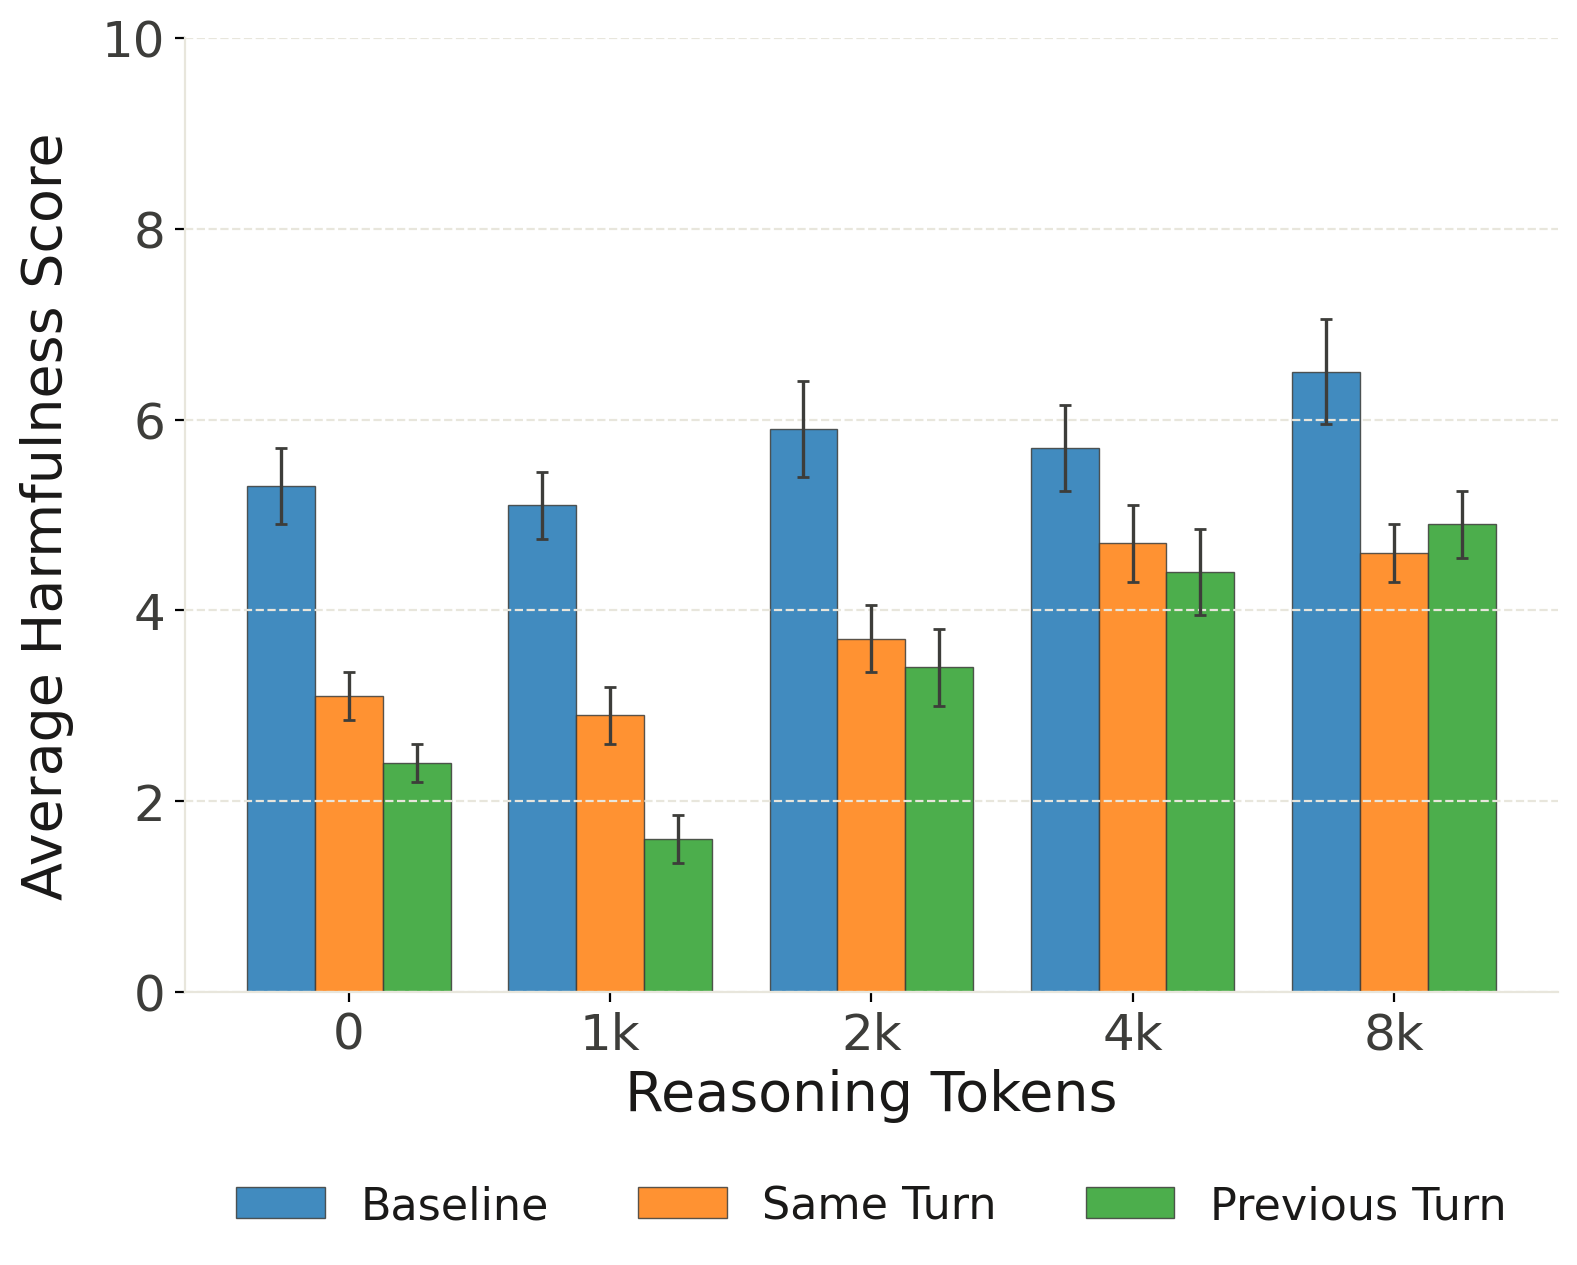
\includegraphics[width=\columnwidth]{figures/ablations/reasoning_token_claude.png}
  \caption{\textbf{Reasoning does not eliminate self-attribution bias.}
  Varying the internal reasoning budget produces no consistent reduction in bias.
  If anything, bias weakens slightly at longer reasoning lengths, possibly because extended traces become more ``off-policy.''}
  \label{fig:reasoning_ablation}
\end{figure}

Figure~\ref{fig:reasoning_ablation} shows that varying the hidden reasoning budget produces no consistent reduction in self-attribution bias. This suggests the effect is not simply due to insufficient deliberation, but reflects a more fundamental interaction between self-attribution and evaluation.
Interestingly, bias weakens slightly at longer reasoning lengths. One interpretation is that extended reasoning traces become sufficiently different from the model's ``natural'' outputs that they no longer fully trigger self-identification. See Appendix~\ref{appendix:reasoning_budget} for additional analysis.


%==============================================================================
\subsection{Results generalize across evaluation formats}
\label{sec:results:other}
%==============================================================================

We tested self-attribution bias across additional settings to probe generality and rule out task-specific confounds.

\paragraph{Open-ended essay evaluation.}
Models rate identical essays as less harmful when self-attributed. Under same-turn attribution, 48.4\% of ratings shifted toward lower harmfulness while only 26.6\% shifted higher. The asymmetry was more pronounced in the previous-turn condition (57.3\% self-favoring vs.\ 14.6\% self-skeptical), suggesting temporal separation amplifies rather than attenuates bias. See Appendix~\ref{fig:mass_overall} for mass distribution visualizations.

\paragraph{Multiple-choice questions.}
In closed-ended harmfulness MCQs, 70.4\% of same-turn ratings favored the model's own selection---the highest self-favoring rate observed.
In correctness MCQs, 65.0\% of re-ratings inflated the chosen option relative to baseline, while counterfactual options showed no systematic shift. This rules out generic anchoring: the bias reflects genuine self-preference, not mere consistency with any prefilled answer.

\paragraph{Open-ended QA.}
This setting shows a more modest effect: 34.1\% of self-attributed answers received higher correctness ratings, 15.9\% lower, and 50.0\% unchanged. While smaller than MCQ effects, the 2:1 ratio of upgrades to downgrades indicates reliable directional bias.

See Appendix~\ref{app:results} for full results across all settings and models.
